\documentclass[11pt, spanish]{article}

\usepackage[spanish]{babel}
\selectlanguage{spanish}
\usepackage[utf8]{inputenc}
\usepackage{graphicx}
\usepackage{fancyhdr}
\usepackage{multicol}
\usepackage{amsmath, amssymb}
\usepackage{enumerate}
\pagestyle{fancy}
\usepackage{tikz}

\tikzset{
  treenode/.style = {shape=rectangle, rounded corners,
                     draw, align=center,
                     top color=white, bottom color=blue!20},
  root/.style     = {treenode, font=\Large, bottom color=red!30},
  env/.style      = {treenode, font=\ttfamily\normalsize},
  dummy/.style    = {circle,draw}
}

\usetikzlibrary{shapes}
\usepackage{xspace}

\newcommand{\A}{\ensuremath{\mathcal{A}}\xspace}
\newcommand{\B}{\ensuremath{\mathcal{B}}\xspace}
\newcommand\pa[1]{\ensuremath{\left(#1\right)}}


\fancyhf{}
\rhead{201111578 \\ 201317343}
\lhead{Sebastián Valencia Calderón \\ Edgar Daniel Gómez}
\rfoot{\thepage}

\begin{document}

\section{VA Discretas y Continuas de Mayor Aplicación}

\begin{enumerate}[(a)]

\item Según estándares FIFA, un balón oficial debe de tener una presión de aire entre
8.5 y 15.6 psi. Si la empresa Tygol establece que una válvula es defectuosa si no logra
mantener dicho estándar de presión, calcule la probabilidad de que una válvula fabricada por
el proveedor sea defectuosa.\\

Sea $X$ la variable aleatoria que representa la presión de aire de un balón luego de 24 horas de fabricado. Por información recolectada y expuesta en el enunciado, se sabe que $X \sim Tri(8.05,\  9.17,\ 17.09)$. Se sabe que un balón posee los estándares considerados como óptimos para un encuentro deportivo sí y sólo sí, la presión de aire de este está entre $8.5$ y $15.6$ psi. La probabilidad de que un balón tomado aletoriamente de la muestra modelada por la variable $X$, sea óptimo para un encuentro deportivo es: $\mathbb{P}(8.5 < X < 15.6)$. La variable y la región correspondiente a la presión de un balón óptimo, se muestran a continuación:

\begin{figure}[h]
    \centering
    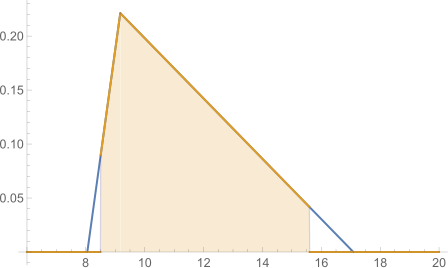
\includegraphics[width=0.6\textwidth]{fig1-1.png}
    \caption{Función de probabilidad normal, horas contra probabilidad}
    \label{fig:prob_dist1}
\end{figure}

$$\mathbb{P}(8.5 < X < 15.6) = \mathbb{P}(X < 15.6) - \mathbb{P}(X < 8.5)$$

La distribución acumulada de una variable aleatoria $X \sim Tri(a,\ c,\ b)$ es:

\[ \mathbb{P}(X < x) = \begin{cases} 
      \frac{(x - a)^2}{(b - a)(c - a)} & a < x < c \\
      1 - \frac{(x - b)^2}{(b - a)(b - c)} & c \leq x < b
   \end{cases}
\]

$$\mathbb{P}(X < 15.6) - \mathbb{P}(X < 8.5) = 0.9689 - 0.0200 = 0.948991$$

La probabilidad de que un balón esté en óptimas condiciones según su aire almacenado es: $0.948991$.

\item ¿Cuál es la probabilidad de que se decida iniciar la producción de los nuevos
balones en la Etapa 1, sin pasar a la Etapa 2?\\

Los eventos de interés en el experimento enunciado, se resumen a continuación como variable aleatorias. Sea $E_{1}$ la variable aleatoria que representa la etapa 1 del proceso de selección, y sea $E_{2}$ la variable que representa el proceso de la segunda y última etapa.

\[ \mbox{Etapa1}(X) = \begin{cases} 
      \mbox{Inicia} & X \leq 2 \\
      \mbox{Etapa2} & 2 < X < 6 \\
      \mbox{Postpone} & X \geq 6
   \end{cases}
\]

\[ \mbox{Etapa2}(X) = \begin{cases} 
      \mbox{Inicia} & E_1 + X \leq 6 \\
      \mbox{Postpone} & E_1 + X > 6
   \end{cases}
\]

\textbf{Etapa 1}: se toma una muestra aleatoria de 50 balones. Si se encuentra un máximo de 2 balones que presenten fallas en las válvulas, se decide iniciar la producción sin pasar a la Etapa 2; si se encuentran al menos 6 balones que presenten fallas en las válvulas, se pospone la producción; de lo contrario, se realiza la Etapa 2 de control de calidad.

\textbf{Etapa 2}: se toma una segunda muestra aleatoria de 100 balones. Si el número de balones que presentan fallas de esta segunda muestra más el número de balones defectuosos de la primera muestra aleatoria no superan las 6 unidades, se da inicio a la producción. De lo contrario, se decide posponer la producción hasta llegar a un acuerdo de garantía con el proveedor de las válvulas.

$$E_1 \sim Bin(p = 1 - 0.948991;\ N = 50)$$
$$E_1 \sim Bin(p = 0.051009;\ N = 50)$$

La producción inicia sin pasar por la etapa dos sí y sólo si $E_1 \leq 2$. 

$$\mathbb{P}(E_1 = k) = \binom{N}{k}p^k(1-p)^{N-k}$$
$$\mathbb{P}(E_1 \leq k) = \sum_{i = \min{\left\{\mathbb{R}[E_1]\right\}}}^{k}  \binom{N}{i}p^i(1-p)^{N-i}$$
$$\mathbb{P}(E_1 \leq 2) = \sum_{i = 0}^{2}  \binom{N}{i}p^i(1-p)^{N-i} $$
$$= \binom{N}{0}p^0(1-p)^{N-0} + \binom{N}{1}p^1(1-p)^{N-1} + \binom{N}{2}p^2(1-p)^{N-2}$$
$$= \binom{50}{0}(1-p)^{50} + \binom{50}{1}p(1-p)^{49} + \binom{50}{2}p^2(1-p)^{48} = 0.527287$$
 
\item ¿Cuál es la probabilidad de que se deba posponer la producción en la Etapa 1, sin
pasar a la Etapa 2?\\

De acuerdo a la explicación, convención y deducción del literal inmediatamente anterior, se pide por la probabilidad:

$$\mathbb{P}(X \geq 6) = 1 - \mathbb{P}(X < 6) = 1 - \mathbb{P}(X \leq 5)$$
$$= 1 - \left[ \sum_{i = 0}^{5}  \binom{N}{i}p^i(1-p)^{N-i} \right] = 1 - 0.95899 = 0.0410086$$

\item Si luego de la primera etapa se sabe que es necesario realizar la Etapa 2 de
control de calidad, ¿cuál es la probabilidad de que se acepte la producción bajo los criterios de
esta etapa?\\

De manera análoga, $E_2 \sim Bin(p = 0.051009;\ N = 100)$. Para que esto ocurra, debe suceder que una vez aceptado el lote en la etapa 1, este sea aceptado en la segunda etapa, para esto, es necesario considerar la desigualdad que implica esto ($E_1 + E_2 \leq 6$), lo cual sólo ocurre si en la etapa uno, $E_1$ tomó alguno de los valores en $\left\{ 3,\ 4,\ 5 \right\}$. Para numerar los posibles resultados o más bien la combinación de resultados se hace uso del siguiente diagráma:

$$E_1 = 3 \Rightarrow E_2 \in \left\{ 0,\ 1,\, 2,\ 3\right\}$$
$$E_1 = 4 \Rightarrow E_2 \in \left\{ 0,\ 1,\, 2\right\}$$
$$E_1 = 5 \Rightarrow E_2 \in \left\{ 0,\ 1\right\}$$

La probabilidad de cada una de las intersecciones ($E_1 = 3 \wedge E_2 \in \left\{ 0,\ 1,\ 2,\ 3 \right\},\ E_1 = 4 \wedge E_2 \in \left\{ 0,\ 1,\ 2\right\},\ E_1 = 5 \wedge E_2 \in \left\{ 0,\ 1\right\}$) es:

$$A = \sum_{i \in \left\{ 0,\ 1,\ 2,\ 3 \right\}} \left[ \left( \binom{50}{3}p^3(1-p)^{47} \right) \times  \left( \binom{100}{i}p^i(1-p)^{100 - i} \right) \right]$$
$$B = \sum_{i \in \left\{ 0,\ 1,\ 2 \right\}} \left[ \left( \binom{50}{4}p^4(1-p)^{46} \right) \times  \left( \binom{100}{i}p^i(1-p)^{100 - i} \right) \right]$$
$$C = \sum_{i \in \left\{ 0,\ 1 \right\}} \left[ \left( \binom{50}{5}p^5(1-p)^{45} \right) \times  \left( \binom{100}{i}p^i(1-p)^{100 - i} \right) \right]$$

$$\mathbb{P}(E_1 \cap E_2) = $$
$$ \sum_{i = 0}^{3} \mathbb{P}(E_1 = 3 \wedge E_2 = i) +  \sum_{i = 0}^{2} \mathbb{P}(E_1 = 4 \wedge E_2 = i)\ + $$
$$ \sum_{i = 0}^{1} \mathbb{P}(E_1 = 4 \wedge E_2 = i) = A + B + C$$
$$0.054134 + 0.0154391 + 0.00235399 = 0.0719271 \Rightarrow$$
$$\mathbb{P}(E_1 \cap E_2) = 0.0719271$$

\item El gerente del área de control de calidad ha decidido recolectar una muestra
aleatoria de 5 balones que presenten fallas en las válvulas, para inspeccionar los aspectos
específicos que ocasionan las fallas. Si el gerente inspecciona uno a uno los balones que
salen de la línea de producción, ¿cuál es la probabilidad de que deban inspeccionar 80
balones hasta completar la muestra requerida?\\

En este literal, se quiere saber cuál es la probabilidad de que el número de balones revisados para completar una colección de cinco balones defectuosos sea 80. La descripción de el experimento, coincide con un modela ajo una variable aleatoria binomial negativa. $X$: Número de balones revisados para completar una colección de cinco balones no óptimos. Por la descripción de la variable aleatoria, $X \sim Bin^{*}(p = 0.051009;\ k = 5)$. 

$$\mathbb{P}(X = x) = \binom{x - 1}{k - 1}p^k(1 - p)^{x - k}$$
$$\mathbb{P}(X = 80) = \binom{80 - 1}{5 - 1}p^5(1 - p)^{80 - 5} = \binom{79}{4}p^5(1 - p)^{75} = 0.010226$$

\item Calcule la probabilidad de que el décimo y el onceavo balón que inspecciona el
gerente sean los dos primeros balones que presenten fallas.\\

Sea $X$ el número de balones que fallan. Entonces, $x = \left\{ 10, 11\right\};\ k = \left\{ 1, 2\right\};\ p = 0.051009$. La pobabilidad de que el décimo balón inspeccionado sea el primero en presentar fallas es $Bin^*(10,\ 1,\ 0.051009)$. La probabilidad de que el onceavo balón inspeccionado sea el segundo en presentar fallas es $Bin^*(11,\ 2,\ 0.051009)$. Dada la independencia de caa inspección, la pobabilidad de que el décimo sea el primero en poseer fallas y el onceavo el segundo en oseer fallas es: 

$$Bin^*(10,\ 1,\ 0.051009) \times Bin^*(11,\ 2,\ 0.051009)$$
$$\binom{10 - 1}{1 - 1}0.051009^1(1 - 0.051009)^{10 - 1} \times \binom{11 - 1}{2 - 1}0.051009^2(1 - 0.051009)^{11 - 2}$$
$$\binom{9}{0}0.051009(1 - 0.051009)^{9} \times \binom{10}{1}0.051009^2(1 - 0.051009)^{9}$$
$$0.0318424 \times 0.0162425 = 0.0005172$$

\item Bajo el contexto del literal $e)$ ¿cuál es el número esperado de balones que no
presentan fallas en las válvulas, que el gerente esperaría encontrar antes de completar su
muestra de 5 balones defectuosos?\\

El valor esperado de la distribución del literal $e)$ pero con la probabilidad de encontrar balones sin defectos. Es decir, dada la distribución $X \sim Bin^{*}(p = 1 - 0.051009;\ k = 5)$. Este valor, corresponde El valor esperado de ésta distribución es:

$$\mu = \frac{k(1 - p)}{p} = $$

\item Se envían 100 balones al proveedor de válvulas para que realice otras pruebas
relacionadas al desgaste de las mismas. Se sabe de antemano que entre los balones
enviados hay 30 que presentan fallas. Calcule la probabilidad de que, si el proveedor toma
una muestra aleatoria de 20 de estos 100 balones, encuentre a lo sumo 6 que presenten
fallas.\\

En total, se seleccionan 20 balones de 100, las formas de hacer esto, es $\binom{100}{20}$. De la selección que se quiere hacer, $x$ balones de los 20, deben presentar fallas, es decir, deben pertenecer a los 30 en total que presentan fallas; mientras que los $20 - x$ restantes, deben ser seleccionados de los 70 totales que no presentan fallas. Se quiere la unión de los eventos mutuamente excluyentes que corresponden a $x \in \left\{ 0,\ 1,\ 2,\ 3,\ 4,\ 5,\ 6 \right\}$. La probabilidad para cada $x$ es:

$$\frac{\binom{30}{x} \times \binom{70}{20 - x}}{\binom{100}{20}}$$

Para todos los $x$:

$$\sum_{i = 0}^{6} \left[ \frac{\binom{30}{i} \times \binom{70}{20 - i}}{\binom{100}{20}} \right] = \frac{8435940105002}{13715194896249} = 0.61508$$

\end{enumerate}

\pagebreak
\section{Proceso de Poisson y Distribución Exponencial}

Dado que el tiempo de llegada entre dos paciente se distribuye de manera exponencial, es
posible definir dos tasa, una para horas pico y otro para horas valle, que esta definidas
como:

$$t \in \left[ 5am - 1pm \right] \Rightarrow \lambda_{5am - 1pm}\ ;\ t = \frac{1}{20} = 0.05\ \frac{pacientes}{minuto}$$
$$t \in \left[ 1apm - 4am \right] \Rightarrow \lambda_{1apm - 4am}\ ;\ t = \frac{1}{45} = 0.022\ \frac{pacientes}{minuto}$$

\begin{enumerate}[(a)]

\item ¿Cuál es la probabilidad de que en la hora pico de urgencias lleguen a lo sumo 20
pacientes?\\

\begin{enumerate}[(I)]

\item Para dar solución a la pregunta en cuestión, se plantea como variable aleatoria
discreta, el número de pacientes que llegan en un determinado intervalo de
tiempo, es decir:
$$\textbf{V.A:} \ \mbox{número de pacientes que llegan en un intervalo de tiempo}. $$

\item Para encontrar la probabilidad de un evento dada la variable aleatoria, es
necesario definir la función de probabilidad por medio de una distribución de
Poisson $p(x,\ \lambda t)$, donde los parámetros $x,\ \lambda t$ son el número de personas que llegan y la tasa de llegada, respectivamente. La distribución que definida de la
siguiente manera:

$$p(x,\ \lambda t) = \frac{e^{-\lambda t}(\lambda t)^x}{x!};\ x \leq 20 \wedge \lambda = \frac{1}{20} = 0.05\ \frac{pacientes}{minuto}$$

\item La probabilidad de que lleguen a lo sumo 20 pacientes está dada por la suma
de las probabilidades de que lleguen de 0 a 20 pacientes, dando como resultado la
siguiente sumatoria:

$$\sum_{x = 0}^{20} \left( \frac{e^{-\lambda t}(\lambda t)^{x}}{x!} \right) = 0.2426$$

\end{enumerate}

\item ¿Cuál es el valor esperado y la varianza del número de pacientes que son
atendidos durante la hora pico en urgencias?

$$\mu = \mathbb{E}(X) = (0.05)(8 \times 60) = 24 \ \frac{pacientes}{hora}$$
$$\sigma ^2 = \mathbb{V}(X) = 24$$

\item ¿Cuál es la probabilidad de que lleguen exactamente 15 pacientes entre las 7:00
a.m. y las 10:00 a.m.?\\

$$\mathbb{P}(X = 15) =  \frac{e^{-0.05 \times 3 \times 60}(0.05 \times 3 \times 60)^{15}}{x!} = 0.01944$$

\item ¿Cuál es la probabilidad de que lleguen por lo menos 6 pacientes entre las 12:00
a.m. y las 5:00 a.m.?\\

Dado que la probabilidad de que $X$ sea mayor a 6 resultaría en una sumatoria
infinita cuya solución estaría dada por una integral impropia, plantearemos la
probabilidad de manera que resulte en una sumatoria finita, como se muestra a
continuación:

$$\mathbb{P}(X \geq 6) = 1 - \mathbb{P}(X < 6)  = 1 - \left[ \sum_{x = 0}^{6} \left( \frac{e^{-\lambda_{1} t}(\lambda_{1} t)^{x}}{x!} \right)\right] = 0.49$$

\item Si entre las 4:00 a.m. y las 10:00 a.m. llegaron 25 pacientes, ¿cuál es la
probabilidad de que entre las 10:00 a.m. y las 12:00 p.m. lleguen menos de 3 pacientes? Por
otro lado ¿cuál es la probabilidad de que lleguen 28 pacientes entre las 4:00 a.m. y las 11:00
a.m.?\\

\begin{enumerate}[(I)]

\item Dado que los eventos son independientes La probabilidad queda definida de la
siguiente manera:

 $$\mathbb{P}(X < 3) = \sum_{x = 0}^{2} \left( \frac{e^{-\lambda_{1} t}(\lambda_{1} t)^{x}}{x!} \right) = 0.0619$$
 
\item Si se sabe que de 4:00am a 10:00am llegaron 25 pacientes entonces queda
encontrar la probabilidad de que entre las 10 y las 11:00am llegue 3 personas:

 $$\mathbb{P}(X = 3) =  \frac{e^{-\lambda_{1} 60}(\lambda_{1} 60)^{3}}{3!} = 0.224 $$

\end{enumerate}

\item Si se sabe que llegaron 30 pacientes entre las 10:00 p.m. y las 4:00 a.m., ¿cuál
es la probabilidad de que 20 pacientes hayan llegado entre la 1:30 a.m. y las 3:15 a.m.?\\

Se trata de una probabilidad condicional dada por los eventos.

$$\textbf{A}:\ X(10 \ pm-4 \ am) = 30$$
$$\textbf{B}:\ X(1:30 \ am-3:15 \ am) = 20$$

La probabilidad solicitada es $\mathbb{P}(B|A)$, sin embargo como el intervalo de B esta
contenido en A, los eventos no son independientes por lo que encontrar su
intersección no es trivial. A pesar de esto, el problema puede ser definido a partir
de intervalos independientes; intervalo “Y” de 10pm a 1:30am, intervalo “X” de
1:35am a 3:15am y el intervalo “Z” de 3:15am hasta las 4am. Dado que la
probabilidad solicitada es que en el intervalo X lleguen 20 personas, es necesario
encontrar la probabilidad de que la suma de los intervalos Y y Z sea 10. Este grupo
de probabilidades queda definido como:

$$\mathbb{P}(X = 20) \times  \sum_{u = 0}^{10} \left[  \mathbb{P}(X = u) \times \mathbb{P}(X = 10 - u)\right] $$
$$\frac{e^{-\lambda_{2} 105}(\lambda_{2} 105)^{20}}{20!} \times \sum_{u = 0}^{10} \left[ \left( \frac{e^{-\lambda_{2} 105}(\lambda_{2} 105)^{u}}{u!}\right) \times \frac{e^{-\lambda_{2} 15}(\lambda_{2} 15)^{10-u}}{(10-u)!} \right]$$

\item Si a las 5:15 a.m. llega el primer paciente de la hora pico a urgencias ¿cuál es la
probabilidad de que el próxima paciente en llegar se demoré más de media hora?\\

\begin{enumerate}[(I)]

\item Para dar solución a la pregunta en cuestión, se plantea como variable aleatoria
continua, el tiempo de llegada entre pacientes.

$$\textbf{VA}: \mbox{tiempo de llegada entre pacientes}$$

\item Para encontrar la probabilidad de un evento dada la variable aleatoria, es
necesario definir la función de probabilidad por medio de una distribución
exponencial $f(X)$, donde el parámetro $X$ es el tiempo. La distribución que
definida de la siguiente manera:
$$f(X) = e^{-\lambda t}(\lambda t);\ x > 30 \wedge \lambda = \frac{1}{20} = 0.05$$

\item La probabilidad de que el próximo paciente llegue en media hora está dada
por:
$$\mathbb{P}(X > 30) = 1 - \mathbb{P}(X \leq 30) = 1 - \int_{0}^{30} e^{-\lambda t}(\lambda t)\ dt = 0.22$$

\end{enumerate}

\item Si a las 12:30 p.m. llega un paciente ¿cuál es la probabilidad de que el tiempo que
se demora el siguiente paciente en llegar al centro de urgencias esté entre 15 y 30 minutos?
$$\mathbb{P}(15 < X < 30) = \int_{15}^{30} e^{-\lambda t}(\lambda t)\ dt = 0.25$$

\item Si a las 12:00 p.m. han llegado 5 pacientes ¿cuál es la probabilidad de que el
próximo paciente llegue exactamente en 20 minutos?
$$\mathbb{P}(X = 0) = 0$$

\item Si a las 8:00 p.m. se sabe que el último paciente llegó hace media hora, ¿cuál es
la probabilidad de que el tiempo de llegada del siguiente paciente a urgencias sea mayor a
una hora?
$$\mathbb{P}(X > 60) = 1 - \mathbb{P}(X \leq  60) = 1 - \int_{0}^{60} e^{-\lambda t}(\lambda t)\ dt = 0.14$$

\end{enumerate}

\pagebreak
\section{Distribución Normal}

\begin{enumerate}[(a)]

\item Si se aborda un bus híbrido o del SITP al azar durante hora pico ¿cuál es la
probabilidad de que en un día seleccionado al azar el tiempo de trayecto sea mayor a 1.5
horas?\\

Sea $X$ la variable aleatoria que representa la demora de un bus híbrido en horas pico sobre las calles 34 y 100. $X \sim \mathcal{N} (\mu , \sigma ^2) = \mathcal{N} (1.25, 0.2^2)$. La gráfica de la distribución normal del enunciado, se muestra acontinuación:

\begin{figure}[h]
    \centering
    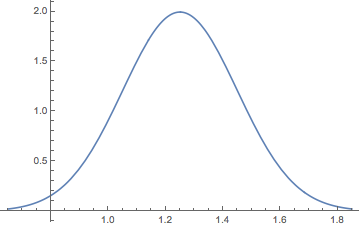
\includegraphics[width=0.6\textwidth]{fig3-1.png}
    \caption{Función de probabilidad normal, horas contra probabilidad}
    \label{fig:prob_dist1}
\end{figure}

Si se quiere saber la probabilidad de que un viaje en un bus cuya ruta se comporte de acuerdo a la descripción, se quiere saber $\mathbb{P}(X > 1.5)$. Lo cual, por propiedades básicas de la teoría de la probabilidad es igual a $1 - \mathbb{P}(X < 1.5)$ para variables aleatorias continuas. Para hallar esto, se estandariza la variable aleatoria $X$, de tal forma:

$$X \sim \mathcal{N} (\mu , \sigma ^2) \Rightarrow Z \sim \mathcal{N} (0,  1)$$
$$1 - \mathbb{P}(X < 1.5) = 1 - \mathbb{P}\left(Z < \frac{1.5 - \mu}{\sigma}\right) = 1 - \mathbb{P}\left(Z < \frac{1.5 - 1.25}{0.2}\right)$$
$$1 - \mathbb{P}(X < 1.5) = 1 - \mathbb{P}\left(Z < 1.25 \right) = 1 - 0.8944 = 0.10565$$

\pagebreak
La probabilidad que se halló, estaba acumulada en:

\begin{figure}[h]
    \centering
    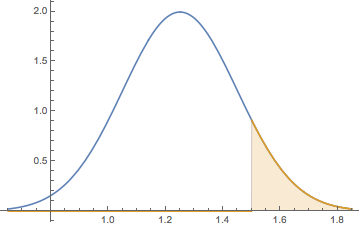
\includegraphics[width=0.6\textwidth]{fig3-2.png}
    \caption{Función de probabilidad normal, horas contra probabilidad.}
    \label{fig:prob_dist2}
\end{figure}

\item Bibiana va tarde a su trabajo y le indicará a su jefe el tiempo máximo que se
tardará en llegar a la oficina. Ella quiere indicarle un tiempo que, con una probabilidad de 0.9,
no exceda el tiempo de recorrido del SITP que acaba de abordar.

Se quiere hallar un $a$ tal que $\mathbb{P}(X < a) = 0.9$. Esto satisface la definición para que con ésta pobabilidad, el tiempo de demora de Bibiana no exceda $a$. Se estandariza este valor:

$$\mathbb{P}\left(Z < \frac{a - \mu}{\sigma} \right) = \mathbb{P}\left(Z < \frac{a - 1.25}{0.2} \right)  = 0.9$$

El valor para cual la variable aleatoria $Z \sim \mathcal{N} (0, 1)$, toma un valor tal que la probabilidad acumulda hasta tal valor sea $0.9$ es, según la tabla de probabilidad acumulada de la Normal estándar es $z = 1.29$. Luego:

$$\frac{a - 1.25}{0.2} = 1.29 \Rightarrow a = (1.29)(0.2) + 1.25 \Rightarrow a = 1.508$$

El tiempo que debe indicar Bibiana es de $1.508$ horas.

\pagebreak
\item Calcule la probabilidad de que un bus seleccionado al azar tenga un tiempo de
trayecto de exactamente una hora.\\

Dado que es una variable aleatoria continua, es imposible calcular la probabilidad puntual de un punto exacto del rango de la distribución, conceptualmente, y analíticamente, este tiende a cero.

$$\mathbb{P}\left(X = 1\right) = 0$$

\item ¿Cuál es la probabilidad de que en un trayecto seleccionado al azar haya tenido
un tiempo de recorrido entre 45 minutos y 1 hora?\\

Se pregunta por la probabilidad de que el timepo transcurrido en un viaje de un bus de la muestra cuyo recorrido se modela haciendo uso de $X$ esté entre 45 minutos y 1 hora exactamente. Es decir:

$$\mathbb{P}(45_{min} < X < 1_{hor}) = \mathbb{P}(0.75_{hor} < X < 1_{hor})$$
 
Por propiedades básicas de las distribuciones de probabilidad:
 
$$\mathbb{P}(0.75_{hor} < X < 1_{hor}) = \mathbb{P}(X < 1_{hor}) - \mathbb{P}(X < 0.75_{hor})$$

Estandarizando la variable $Z \sim \mathcal{N} (0, 1)$, se tiene:

\begin{equation}
    \begin{aligned}
    \mathbb{P}\left(Z < \frac{1 - \mu}{\sigma} \right) - \mathbb{P}\left(Z < \frac{0.75 - \mu}{\sigma} \right) =
    \\
    \\
     \mathbb{P}\left(Z < \frac{1 - 1.25}{0.2} \right) - \mathbb{P}\left(Z < \frac{0.75 - 1.25}{0.2} \right) = 
     \\
     \\
     \mathbb{P}\left(Z < -1.25 \right) - \mathbb{P}\left(Z < -2.5 \right) =
     \\
     \\
     \left[ 1 -  \mathbb{P}\left(Z < 1.25 \right) \right] - \left[ 1 - \mathbb{P}\left(Z < 2.5 \right) \right] = 
     \\
     \\
      -\mathbb{P}\left(Z < 1.25 \right) +  \mathbb{P}\left(Z < 2.5 \right) =
      -0.8944 + 0.9928 
      \\
      = 0.0994401
\end{aligned}
\end{equation}

\pagebreak
La probabilidad que se halló, estaba acumulada en:

\begin{figure}[h]
    \centering
    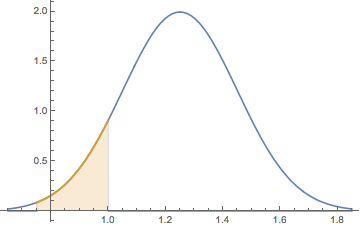
\includegraphics[width=0.6\textwidth]{fig3-3.png}
    \caption{Gráfica de probabilidad de que se llege con un timepo entre 45 minutos y 1 hora.}
    \label{fig:prob_dist2}
\end{figure} 

\item Calcule el valor de la constante $c$ que garantiza que, con probabilidad de 0.90, el
tiempo de recorrido de un bus seleccionado al azar estará intervalo $\left[ 1.25 - c,\ 1.25 + c\right]$.\\

El valor pedido, es un $c$ tal que para algún $X$, la probabilidad de que esté entre $1.25 - c$ y $1.25 + c$ sea $0.90$. Por principios básicos de probabilidad y de distribuciones de probabilidad:

\begin{equation}
    \begin{aligned}
   \mathbb{P}\left(1.25 - c < X < 1.25 + c \right) = 0.9 \Rightarrow   \\
  \mathbb{P}\left(X < 1.25 + c\right) -   \mathbb{P}\left(X < 1.25 - c\right) = 0.9 \Rightarrow\\
  \mbox{Al estandarizar se obtiene:} \\
  \mathbb{P}\left(Z < \frac{1.25 + c - \mu}{\sigma} \right) - \mathbb{P}\left(Z < \frac{1.25 - c - \mu}{\sigma} \right) = 0.9 \Rightarrow \\
  \mathbb{P}\left(Z < \frac{1.25 + c - 1.25}{0.2} \right) - \mathbb{P}\left(Z < \frac{1.25 - c - 1.25}{0.2} \right) = 0.9 \Rightarrow  \\
  \mathbb{P}\left(Z < \frac{c}{0.2} \right) - \mathbb{P}\left(Z < \frac{- c}{0.2} \right) = 0.9 \\
\end{aligned}
\end{equation}

\pagebreak
Por propiedades de las distribuciones normales

$$  \mathbb{P}\left(Z < \frac{c}{0.2} \right) - \left[ 1 - \mathbb{P}\left(Z < \frac{c}{0.2} \right) = 0.9 \right] $$
$$  \mathbb{P}\left(Z < \frac{c}{0.2} \right) - 1 + \mathbb{P}\left(Z < \frac{c}{0.2} \right) = 0.9 $$
$$  2\left(\mathbb{P}\left(Z < \frac{c}{0.2} \right)\right) - 1  = 0.9 \Rightarrow \mathbb{P}\left(Z < \frac{c}{0.2} \right) = \frac{1.9}{2} = 0.95$$

Según la tabla de distribución normal estándar, el primer valor $z$ para el cual $\mathbb{P}\left(Z < z \right) = 0.9$ es $1.65$. Luego, $\frac{c}{2} = 1.65 \Rightarrow c = 0.33$.



\end{enumerate}

\pagebreak
\section{Función Generatriz de Momentos}

\begin{enumerate}[(a)]

\item ¿Cuál es el número esperado de fallas en las máquinas durante un mes?\\

Como $\Psi_{X}(t) = e^{6 \times \left( e ^{t} - 1 \right)}$ es la función generatriz de momentos para la variable aleatoria que representa el número de fallas mensuales que tiene la máquina, y por la teoría se sabe que $\Psi_{X}^r(t = 0) = \mathbb{E}(X^r)$; entonces el primer momento central equivale a $\mathbb{E}(X^1) = \mathbb{E}(X)$.

$$\Psi'_{X}(t) = 6 \times e ^{6 \times (-1 + e^t) + t}$$
$$\Psi'_{X}(0) = 6 \times e ^{6 \times (-1 + e^0) + 0} = 6 \times e ^{6 \times (-1 + 1)} = 6 \times e ^{0} = 1$$

\item ¿Cuál es la varianza del número de fallas en las máquinas durante un mes?\\

Como $\Psi_{X}(t) = e^{6 \times \left( e ^{t} - 1 \right)}$ es la función generatriz de momentos para la variable aleatoria que representa el número de fallas mensuales que tiene la máquina, y por la teoría se sabe que $\Psi_{X}^r(t = 0) = \mathbb{E}(X^r)$; entonces el segundo momento central equivale a $\mathbb{E}(X^2)$.

$$\Psi'_{X}(t) = 6 \times e ^{6 \times (-1 + e^t) + t}$$
$$\Psi''_{X}(t) = 6 \times e^{6 \times \left(e^t-1\right)+t} \times \left(6 \times e^t+1\right)$$
$$\Psi''_{X}(0) = 6 \times e^{6 \times \left(e^0-1\right)+0} \times \left(6 \times e^0+1\right) = 6 \times e^{6 \times \left(1-1\right)+0} \times \left(6 \times 1+1\right)$$
$$\Psi''_{X}(0) = 6 \times e^{0} \times 7 = 6 \times 7 = 42 = \mathbb{E}(X^2)$$
\begin{center}
	\line(1,0){300}
\end{center}
$$\mathbb{V}(X) = \mathbb{E}[X^2] - \mathbb{E}[X]^2 = \Psi''_{X}(0) - (\Psi'_{X}(0))^2 $$
$$\mathbb{V}(X) = 42 - 6^" = 42 - 36 = 6 $$

\item Halle su función generatriz de momentos. Muestre todo el procedimiento.\\

Sea $f_{Y}(y) : \mathbb{R} \mapsto \mathbb{R}$, una función definida por la expresión $f_{Y}(y) = 1/20 \iff y \in (1, 20) \subset \mathbb{R} \wedge f_{Y}(y) = 0 \iff y \notin (1, 20) \subset \mathbb{R}$. Sea $g(t) = e^{t \times y}$, definida sobre $\mathbb{R}$ para todo intervalo de definición de la variable $y$. El producto funcional de ambas funciones, se define através de la variable $y$, por lo que las porciones donde $y$ valfa cero sobre algun intervalo de por lo menos una de las funciones, entonces en el mismo intervalo, el producto funcional es cero. Acontinuación se ilustra el producto funcional de las funciones definidas en este párrafo sobre un intervalo de interés.

\[ f_{Y}(y) = \begin{cases} 
      \frac{1}{20} & 0 < x < 20 \\
      0 & d.l.c
   \end{cases}
\]

$$g(t) = e^{t \times y}$$

\begin{figure}[h]
    \centering
    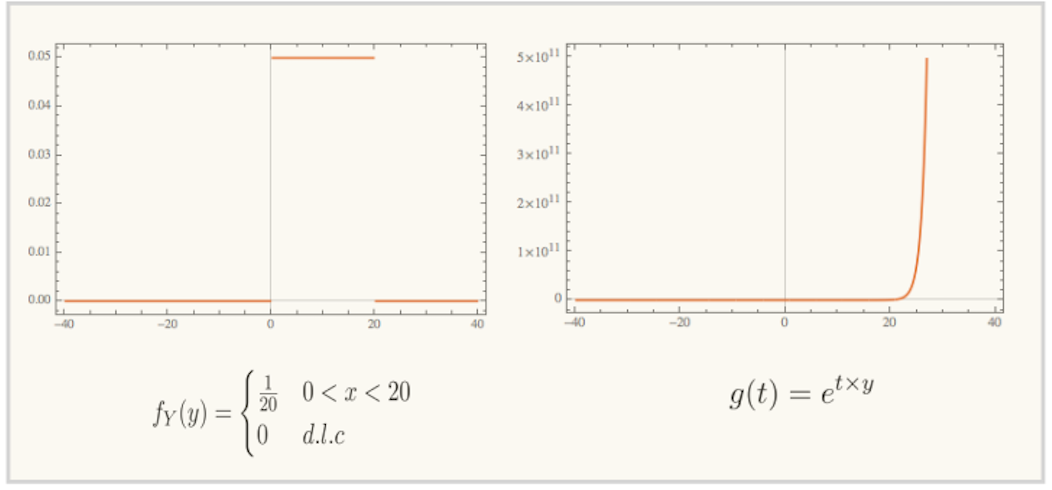
\includegraphics[width=1\textwidth]{fig4-1.png}
    \caption{Función de distribución de probabilidad y función para la generación de momentos centrales de una distribución.}
    \label{fig:prob_dist2}
\end{figure}

$$\Psi_{Y}(t) = \int_{- \infty}^{\infty} \left( e^{y \times t} \times f_{Y}(y)\right)\ dy = \int_{\mathbb{R}[Y]} \left( e^{y \times t} \times f_{Y}(y)\right)\ dy$$
$$\Psi_{Y}(t) = \int_{0}^{20} \left( e^{y \times t} \times f_{Y}(y)\right)\ dy = \int_{0}^{20} \left( e^{y \times t} \times \frac{1}{20}\right)\ dy$$
$$\Psi_{Y}(t) = \frac{1}{20} \int_{0}^{20} e^{y \times t}\ dy = \frac{1}{20} \left[\left.   \frac{e^{t \times y}}{t} \right|_{y=0}^{y = 20}
 \right] = \frac{1}{20} \left[\frac{e^{20 \times t}}{t} -  \frac{e^{0 \times t}}{t} \right]$$
$$\Psi_{Y}(t) = \frac{1}{20} \left[\frac{e^{20 \times t} - e^{0 \times t}}{t} \right] = \frac{1}{20} \left[\frac{e^{20t} - 1}{t} \right] = \frac{e^{20t} - 1}{20t} $$

\end{enumerate}

\end{document}